\documentclass[11pt,fleqn,twoside]{article}
\usepackage{makeidx}
\makeindex
\usepackage{palatino} %or {times} etc
\usepackage{plain} %bibliography style 
\usepackage{amsmath} %math fonts - just in case
\usepackage{amsfonts} %math fonts
\usepackage{amssymb} %math fonts
\usepackage{lastpage} %for footer page numbers
\usepackage{fancyhdr} %header and footer package
\usepackage{mmpv2} 
\usepackage{url}
\usepackage{float}

% the following packages are used for citations - You only need to include one. 
%
% Use the cite package if you are using the numeric style (e.g. IEEEannot). 
% Use the natbib package if you are using the author-date style (e.g. authordate2annot). 
% Only use one of these and comment out the other one. 
\usepackage{cite}
\usepackage[parfill]{parskip}
%\usepackage{natbib}

\begin{document}

\name{Aidan Wynne Fewster}
\userid{awf1}
\projecttitle{NHS Wales injectable medicines guide Android application}
\projecttitlememoir{NHS Wales Android application} %same as the project title or abridged version for page header
\reporttitle{Design Specification}
\version{0.8}
\docstatus{Draft}
\modulecode{CS39440}
\degreeschemecode{G400}
\degreeschemename{Computer Science}
\supervisor{Andrew Starr} % e.g. Neil Taylor
\supervisorid{aos}
\wordcount{}

%optional - comment out next line to use current date for the document
%\documentdate{10th February 2014} 
\mmp

\setcounter{tocdepth}{3} %set required number of level in table of contents


%==============================================================================
\section{Introduction}
%==============================================================================
\subsection{Purpose of this document}
%==============================================================================\
The purpose of the document is to provide documentation for the architectural design of the NHS Wales injectable medicines guide Android application.  It will show the class's which should be created and the methods within them, as well as how they're linked, this will be achieved through a class diagram. This document will also outline the project user interface design through UI mock-up wireframes.


%==============================================================================
\subsection{Project overview}
%==============================================================================
The main focus of this project is to produce a application for Android which will aid NHS medical staff in obtaining information on injectable medicines. The user will be able to search through a list of drugs by there title. Upon selecting a drug they will be able to view a detailed monograph for that drug. User will also be able to calculate dosage and infusion rates using the application.
\newpage
%==============================================================================
\section{Architectural design}
%==============================================================================
This section will contain the architectural for the mobile application. This section will include a use case diagram and a class diagram for the system.

%==============================================================================
\subsection{Use case diagram}
%==============================================================================
\begin{figure}[H]
\centering
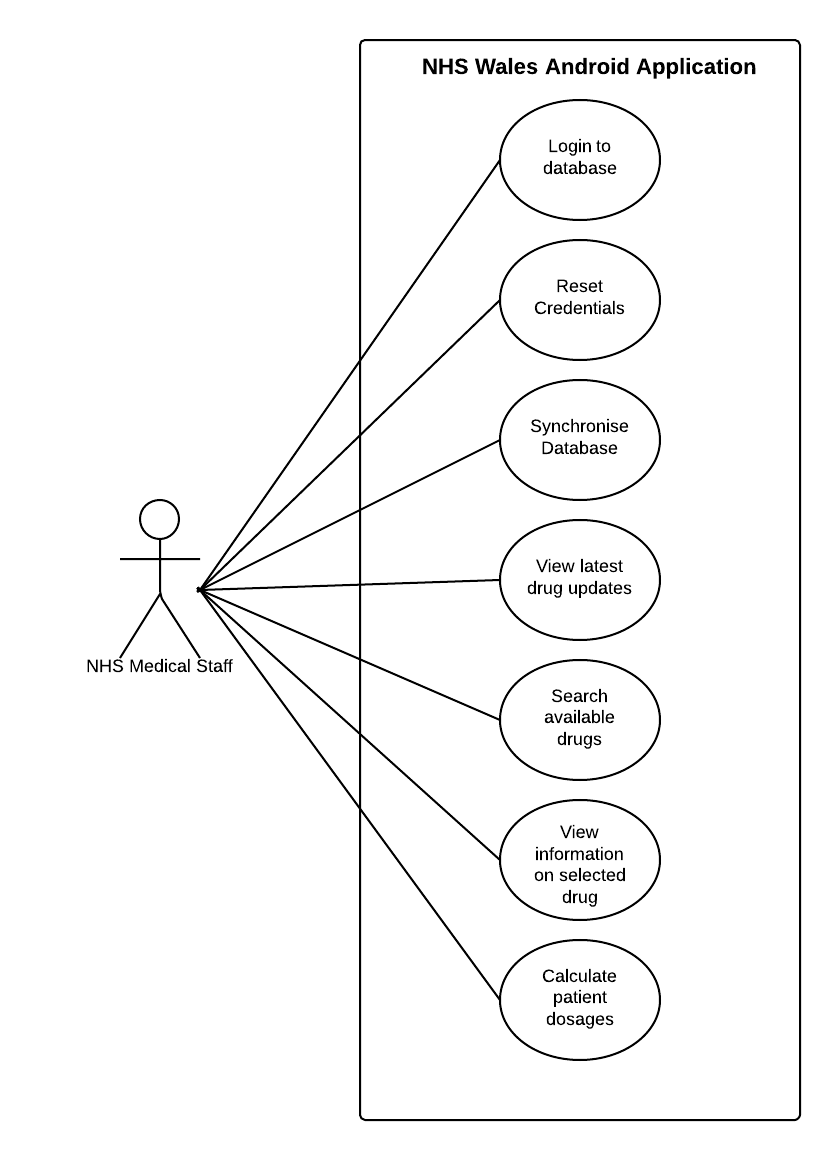
\includegraphics[width=5.5in]{useCase}
\caption{Use case diagram for the NHS application}
\end{figure}
%==============================================================================
\subsubsection{Use case descriptions}
%==============================================================================
\begin{description}
	\item[Login to database]  A user will be able to authenticate themselves with the database using their NHS login credentials.
	\item[Synchronise database] Upon authenticating themselves the user will be able to download a complete copy of the available database to their device.
	\item[View latest drug updates] The user will how many monographs have been added or removed from the live database since they last synchronised their local one.
	\item[Search available drugs] The user will be able to easily search through all the drugs within the database. The search will automatically suggest suitable results.
	\item[View information on selected drug] Upon selecting a drug the user will be able to view a monograph for that drug. They will be able to select each section of the monograph they would like to read.
	\item[Calculate patient dosages] The user will be able to calculate the infusion rate and dosage for a given patient. This information will be validated for user input error. 
\end{description}
\newpage
%==============================================================================
\subsection{Class diagram}
%==============================================================================
\begin{figure}[H]
\centering
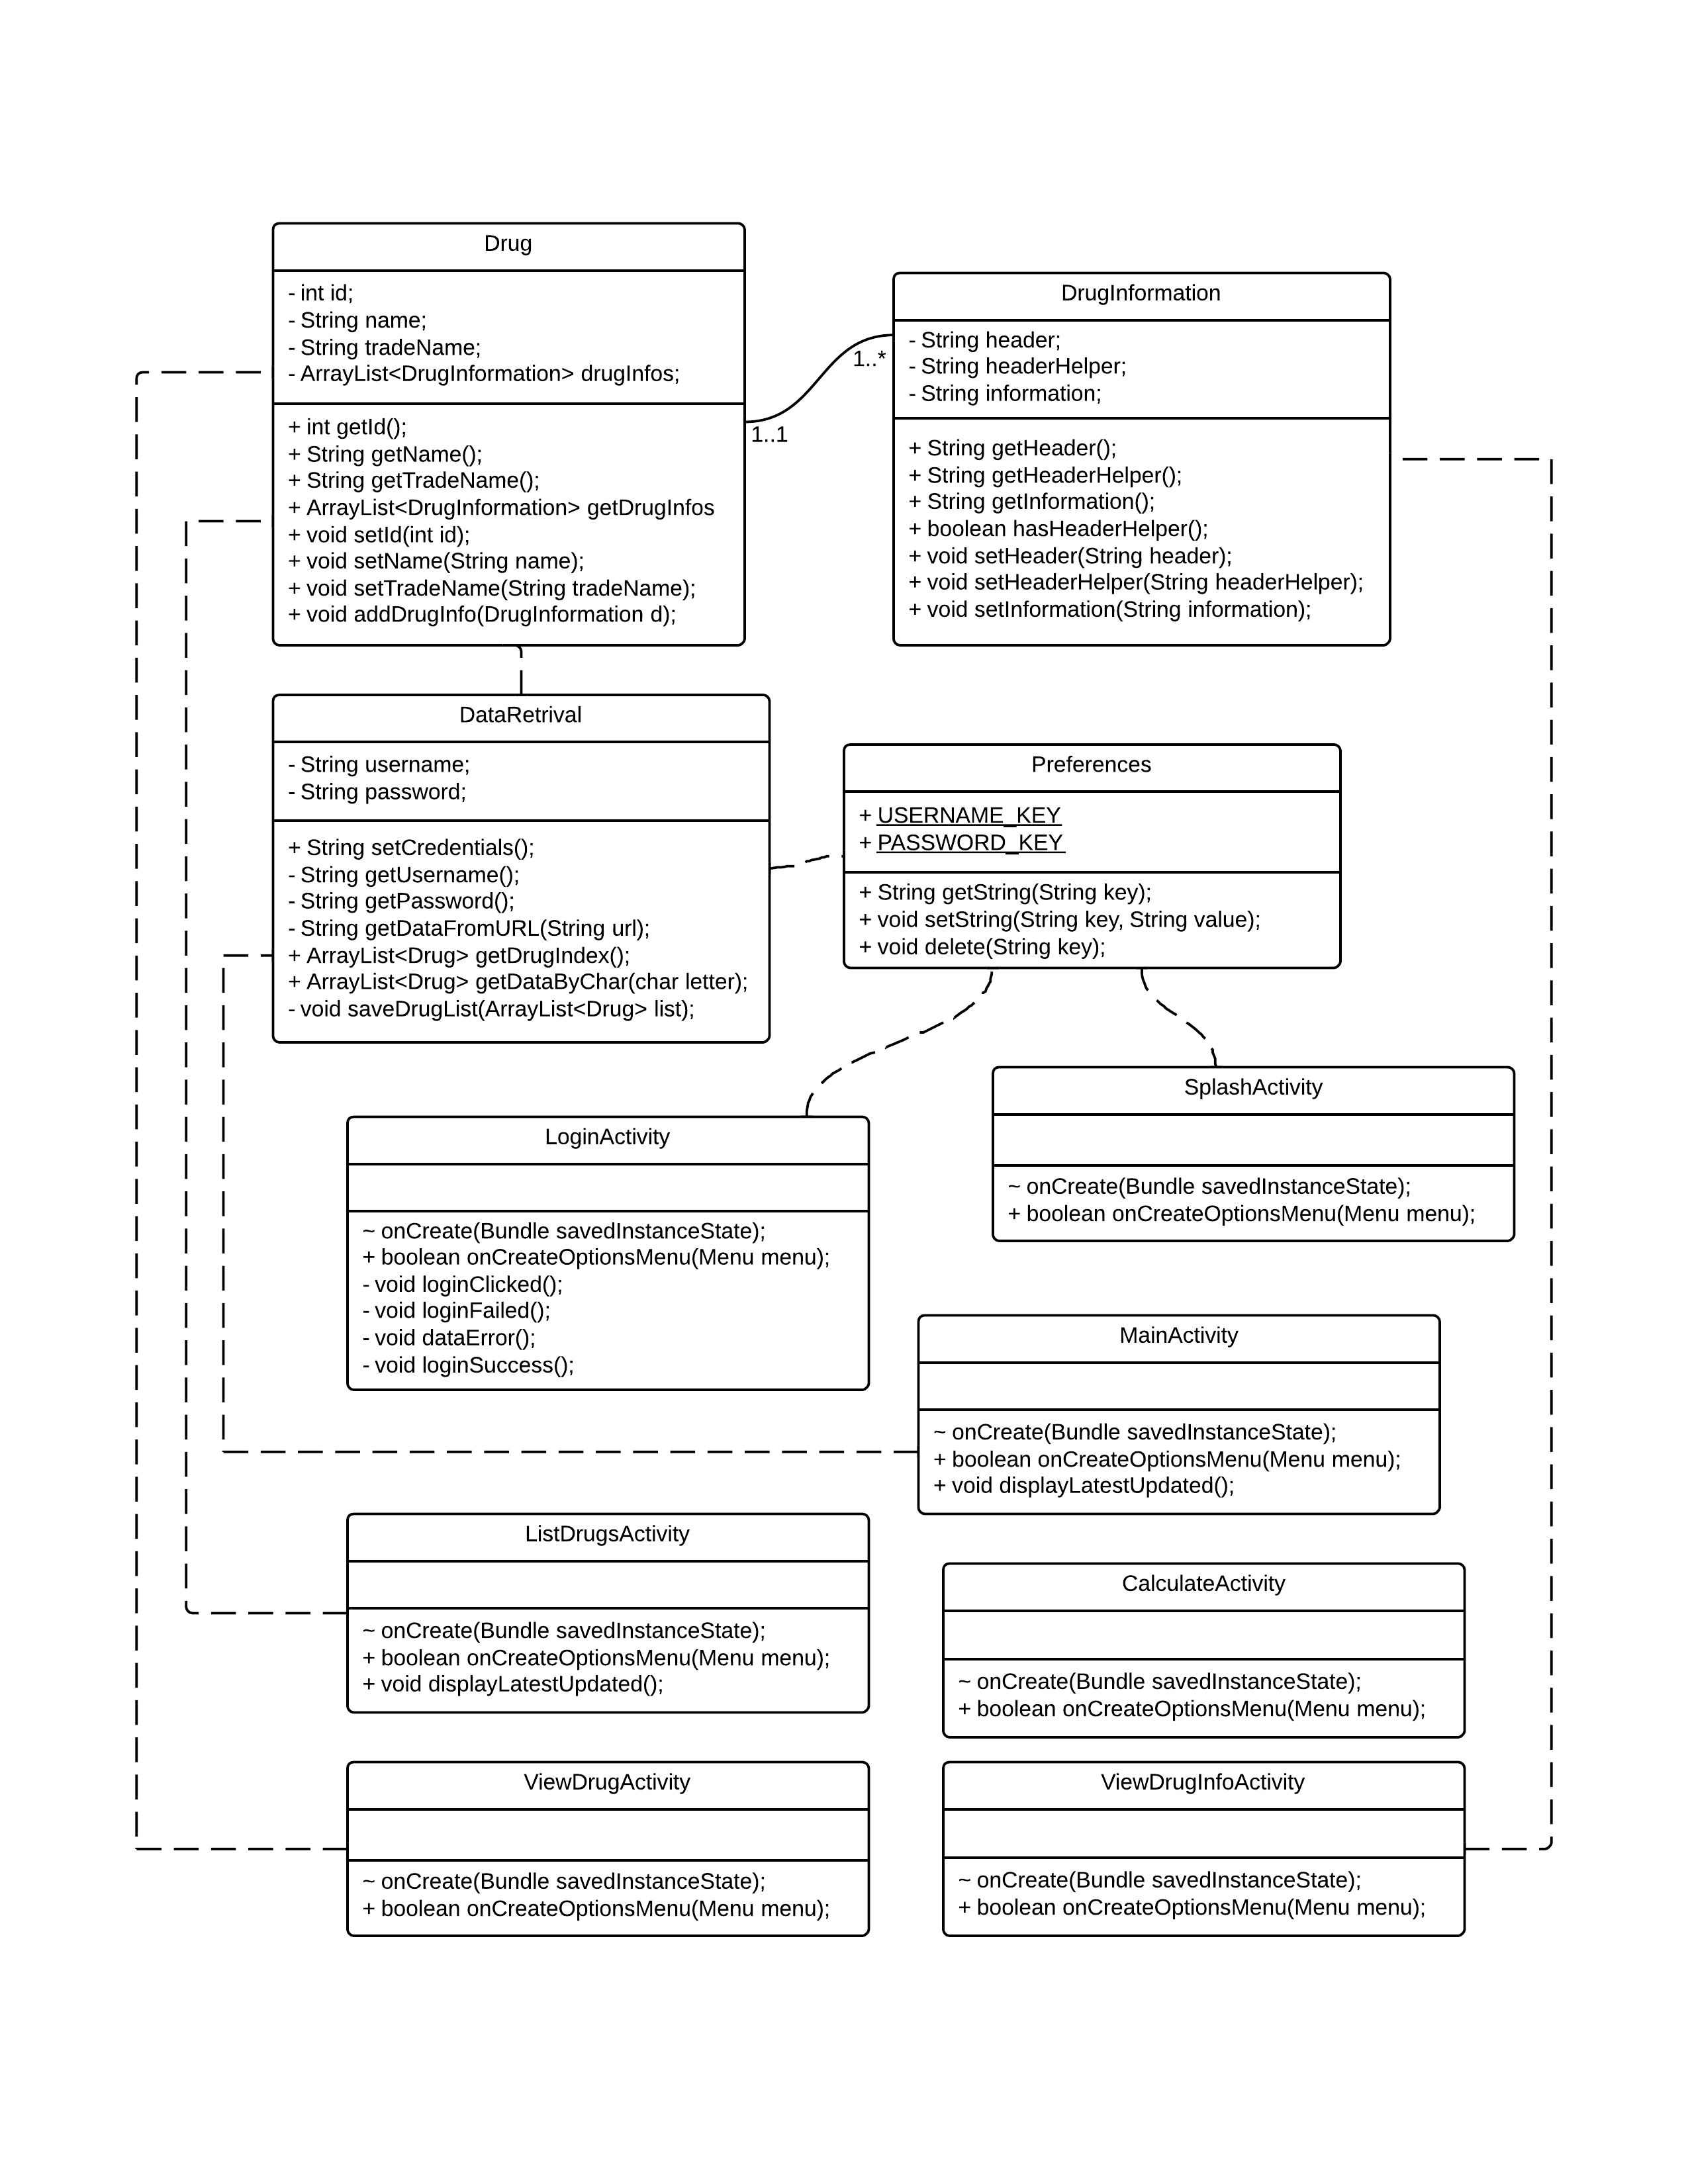
\includegraphics[width=6.5in]{classDiagram}
\caption{Use case diagram for the NHS application}
\end{figure}

%==============================================================================
\subsubsection{Class diagram descriptions}
%==============================================================================
\begin{description}
	\item[Drug] This class represents a drug in the database
	\item[DrugInformation] This class represents a piece of the monographs information about the drug.
	\item[DataRetrival] This class is responsible for authenticating the user and synchronising the local database with the live database.
	\item[Preferences] This class is responsible for accessing the SharedPreferences of the application. It will be used to store and retrieve preferences
	\item[SlashActivity] This is the loading screen when the app first launches
	\item[LoginActivity] This is the activity which the user will use to authenticate themselves
	\item[MainActivity] This class for the main activity, this activity will alert the user of any changes within the live database as well as let the user update their database and begin searching.
	\item[ListDrugsActivity] Class for the list drugs activity, this activity will list all drugs stored in the database, allowing users to search through them.
	\item[ViewDrugActivity] Class for the view drug activity, this activity will display simple information about the drug and allow the user to navigate to detailed information
	\item[ViewDrugInfoActivity] Class for the drug information activity, this activity will display detailed information on a specific piece of the drugs monograph.
	\item[CalculateActivity] Class for the calculate activity, this activity will allow the user to calculate dosage and infusion rates for a patient.

\end{description}

\end{document}
